\documentclass[journel,12pt,twocoloums]{IEEEtran}

\title{Assignment 5-Probability and Random Variable}
\author{Annu-EE21RESCH01010}
\date{13 January 2020}

\usepackage{amsthm}
\usepackage{graphicx}
\usepackage{mathrsfs}
\usepackage{txfonts}
\usepackage{stfloats}
\usepackage{pgfplots}
\usepackage{cite}
\usepackage{cases}
\usepackage{mathtools}
\usepackage{caption}
\usepackage{enumerate}	
\usepackage{enumitem}
\usepackage{amsmath}
\usepackage[utf8]{inputenc}
\usepackage[english]{babel}
\usepackage{multicol}
%\usepackage{xtab}
\usepackage{longtable}
\usepackage{multirow}
%\usepackage{algorithm}
%\usepackage{algpseudocode}
\usepackage{enumitem}
\usepackage{mathtools}
\usepackage{gensymb}
\usepackage{hyperref}
%\usepackage[framemethod=tikz]{mdframed}
\usepackage{listings}
    %\usepackage[latin1]{inputenc}                                 %%
    \usepackage{color}                                            %%
    \usepackage{array}                                            %%
    \usepackage{longtable}                                        %%
    \usepackage{calc}                                             %%
    \usepackage{multirow}                                         %%
    \usepackage{hhline}                                           %%
    \usepackage{ifthen}                                         %%
  \providecommand{\nCr}[2]{\,^{#1}C_{#2}}
  \providecommand{\nPr}[2]{\,^{#1}P_{#2}}
  \lstset{
%language=C,
frame=single, 
breaklines=true,
columns=fullflexible
}

 \begin{document}
 \maketitle
\textbf{Download latex code from here-}\\
\begin{lstlisting}
 https://github.com/annu100/AI5002-Probability-and-Random-variables/tree/main/ASSIGNMENT_5
 \end{lstlisting}
 \textbf{download python code from here}\\
 \begin{lstlisting}
  https://github.com/annu100/AI5002-Probability-and-Random-variables/blob/main/ASSIGNMENT_5/assignment_5.py
 \end{lstlisting}
 \section{Problem Statement-Problem 4.10}
Two dice, one blue and one grey, are thrown
at the same time.
\begin{enumerate}
\item
Complete Table 4.1.1.
\begin{center}
    \begin{tabular}{|c|c|}
    \hline
    2 & $\frac{1}{36}$\\
    \hline
    3 & --- \\
    \hline
    4 & --- \\
    \hline
    5 & --- \\
    \hline
    6 & --- \\
    \hline
    7 & -- \\
    \hline
    8 & $\frac{5}{36}$ \\
    \hline
    9 & --- \\
    \hline
    10 & --- \\
    \hline
    11 & --- \\
    \hline
    12 & $\frac{1}{36}$ \\
    \hline
    \end{tabular}
\end{center}
\item
A student argues that there are 11 possible
outcomes 2, 3, 4, 5, 6, 7, 8, 9, 10, 11 and
12. Therefore, each of them has a probability
1
11 . Do you agree with this argument? Justify
your answer.
\end{enumerate}
\section{Solutions}
Since we know ,the possible outcomes when a pair of two dices are thrown.
Therefore,In a throw of pair of dice, blue and grey, total no of possible outcomes=36(6×6) which are
[(1,1)(1,2)(1,3)(1,4)(1,5)(1,6) \\

(2,1)(2,2)(2,3)(2,4)(2,5)(2,6) \\

(3,1)(3,2)(3,3)(3,4)(3,5)(3,6) \\

(4,1)(4,2)(4,3)(4,4)(4,5)(4,6) \\

(5,1)(5,2)(5,3)(5,4)(5,5)(5,6) \\

(6,1)(6,2)(6,3)(6,4)(6,5)(6,6)]\\


$E_2$ $\to$ \text{ event of getting sum as 2}\\
No. of favorable outcomes =1  (i.e.,(1,1))\\

P($E_2$)=$\frac{1}{36}$\\


$E_3$ $\to$ \text{ event of getting sum as 3}\\

No. of favorable outcomes =2  (i.e.,(1,2)(2,1))\\

P($E_3$)=$\frac{2}{36}$\\
$E_4$ $\to$ \text{ event of getting sum as 4}\\

No. of favorable outcomes =3  (i.e.,(3,1)(2,2)(1,3))\\

P($E_2$)=$\frac{3}{36}$\\
$E_5$ $\to$ \text{ event of getting sum as 5}\\

No. of favorable outcomes =4 (i.e.,(1,4)(2,3)(3,2)(4,1))\\

P($E_5$)=$\frac{4}{36}$\\
$E_6$ $\to$ \text{ event of getting sum as 6}\\

No. of favorable outcomes =5(i.e.,(1,5)(2,4)(3,3)(4,2)(5,1))\\

P($E_6$)=$\frac{5}{36}$\\

$E_7$ $\to$ \text{ event of getting sum as 7}\\

No. of favorable outcomes =6  (i.e.,(1,6)(2,5)(3,4)(4,3)(5,2)(6,1))\\

P($E_7$)=$\frac{6}{36}$\\
$E_8$ $\to$ \text{ event of getting sum as 8}\\

No. of favorable outcomes =5  (i.e.,(2,6)(3,5)(4,4)(5,3)(6,2))\\

P($E_8$)=$\frac{6}{36}$\\
$E_9$ $\to$ \text{ event of getting sum as 9}\\

No. of favorable outcomes =4  (i.e.,(3,6)(4,5)(5,4)(6,3))\\
P($E_9$)=$\frac{4}{36}$\\
$E_10$ $\to$ \text{ event of getting sum as 10} \\

No. of favorable outcomes =3  (i.e.,(4,6)(5,5)(6,4))\\
P($E_10$)=$\frac{3}{36}$\\
 
$E_11$ $\to$ \text{ event of getting sum as 11}\\

No. of favorable outcomes =2,(i.e.,(6,5)(5,6))\\
P($E_11$)=$\frac{2}{36}$\\
 
$E_12$ $\to$ \text{ event of getting sum as 12}\\

No. of favorable outcomes =1,(i.e.,(6,6))\\
P($E_12$)=$\frac{1}{36}$\\

From the figure(table) we can see that the outcomes are not equally likely - we see that, there is different probability for different outcome.\\
Complete Table 4.1.1.
\begin{center}
    \begin{tabular}{|c|c|}
    \hline
    2 & $\frac{1}{36}$\\
    \hline
    3 & $\frac{1}{18}$\\
    \hline
    4 & $\frac{1}{12}$ \\
    \hline
    5 & $\frac{1}{9}$ \\
    \hline
    6 & $\frac{5}{36}$ \\
    \hline
    7 & $\frac{1}{6}$\\
    \hline
    8 & $\frac{5}{36}$ \\
    \hline
    9 & $\frac{1}{9}$\\
    \hline
    10 & $\frac{1}{12}$\\
    \hline
    11 & $\frac{1}{18}$ \\
    \hline
    12 & $\frac{1}{36}$ \\
    \hline
    \caption{\textbf{Sum of numbers on 2 dice and their probability}}
    \label{tab:my_label}
    \end{tabular}
\end{center}

\begin{figure}

\caption{grapgh for probability of sum of 2 numbers on 2 dice}
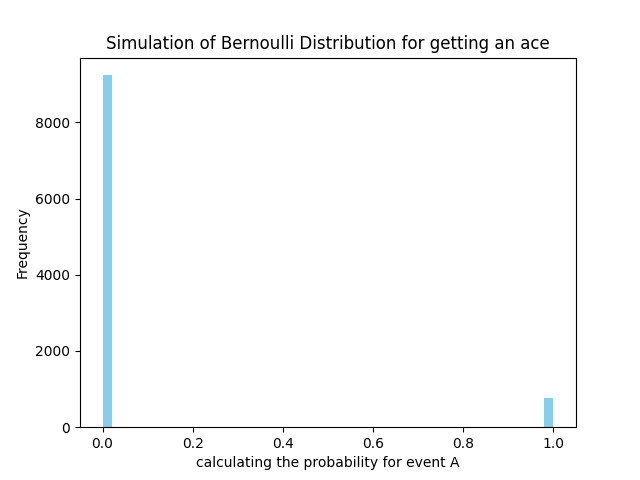
\includegraphics[width=\columnwidth] {Figure_1.png}
\textbf{Above is is the graph of probability for getting sum of two numbers appearing on 2 dices versus possible sums }\\
\end{figure}


\end{document}
        

